\section{Identifikation}
\begin{xltabular}{\linewidth}{|l|l|}
	\hline
	Auftragsnummer & 
	\\\hline
	Auftragsbezeichnung & <Auftragsbezeichnung>
	\\\hline
\end{xltabular}
\label{tab:IdentifikationTable}

\section{Beschrieb des Ablaufs der Arbeit}
Für mein Projekt, das sich auf die Erforschung und Implementierung von Convolutional Neural Networks (CNN) und allgemeinen neuronalen Netzwerken konzentrierte, habe ich mich eigenständig auf eine umfassende Recherche eingelassen. Die Frist war die einzige Vorgabe, was mir die Freiheit liess, meine Interessen vollständig zu verfolgen. Grundlagenwissen zu CNNs und neuronalen Netzwerken sammelte ich durch sorgfältige Recherche auf renommierten Plattformen wie Medium, IBM, Geekflare, der Stanford University, und Database Camp. Bei der Lösung spezifischer Softwareprobleme erwiesen sich Stack Overflow, GitHub Copilot und ChatGPT, sowie die Dokumentationen der verwendeten Abhängigkeiten und Cppreference als unverzichtbare Ressourcen. Der Datensatz, der für das Training des Netzwerks verwendet wurde, stammt von Yann LeCun’s MNIST-Datenbank, einem Standardbenchmark in der Branche.
\\
Die Visualisierung des Projekts erfolgte durch die Erstellung von Ablaufdiagrammen, die sowohl den Prozess als auch die Struktur der Architektur eines neuronalen Netzwerks darstellen, sowie einem Klassendiagramm, das die objektorientierte Struktur der Implementierung verdeutlicht. Da keine Datenbank beteiligt war, wurde kein Entity-Relationship-Modell (ERM) benötigt.
\begin{figure}[H]
	\centering
		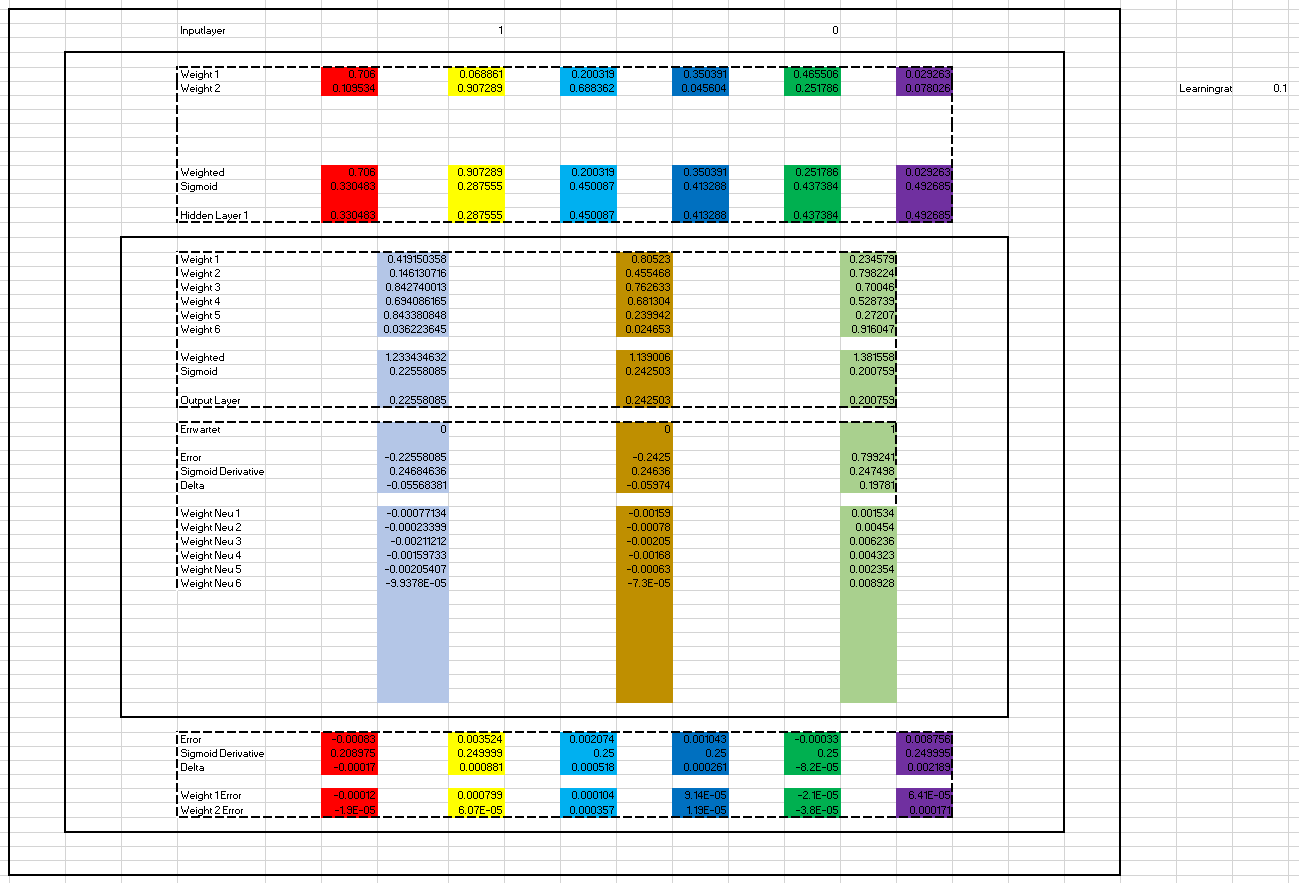
\includegraphics[width=\linewidth]{visualisierungKI.png}
		\caption{Meine Visualisierung eines neuronalen Netzwerkes in Excel.}
	\label{fig:visualisierungKI}
\end{figure}
\\
Die Entscheidung, das Projekt in C++ zu entwickeln, war nicht zufällig, sondern eine bewusste Wahl, die von mehreren Schlüsselfaktoren beeinflusst wurde. Zunächst ist C++ bekannt für seine aussergewöhnliche Leistungsfähigkeit und Effizienz\footnote{Zeigler, 1995; Hudak, 1994}, was es zur idealen Sprache für rechenintensive Anwendungen wie neuronale Netzwerke macht. Meine persönliche Vorliebe für C++ spielte ebenfalls eine Rolle. Überdies eröffnete die Wahl von C++ die Möglichkeit, in Zukunft die Verarbeitungsgeschwindigkeit durch die Einbindung von GPU-Berechnungen zu steigern. Dies wäre ein entscheidender Vorteil für die Skalierung und Effizienz des Projekts. Entwickelt wurde das Ganze unter Windows 11 und Manjaro Linux, einem Arsch-basierten Betriebssystem, mit CLion, einer IDE von JetBrains. Diese Entwicklungsumgebung wurde speziell wegen ihrer Benutzerfreundlichkeit und Cross-Plattform-Unterstützung ausgewählt, was einen nahtlosen Entwicklungsprozess auf verschiedenen Systemen ermöglichte. 
\\
Die Durchführung der Softwaretests erfolgte mittels des Google Test Frameworks, wodurch eine gründliche Prüfung jeder Klasse gewährleistet wurde. Dieser Ansatz trug entscheidend zur Stabilität und Funktionsfähigkeit des entwickelten Systems bei. Obwohl es keinen direkten Kunden für das Projekt gab, entschied ich mich dafür, den Quellcode auf Plattformen wie GitHub und GitLab zu teilen. Dieser Schritt diente nur der Demonstration meiner Arbeit und nicht dem Anstossen von Diskussionen, da dieses Projekt schon vielfach implementiert wurde. Es ist schliesslich das Einsteigerprojekt für Maschine Learning.

\section{Gemachte Erfahrungen}
\subsection{Im Bezug auf die ausgeführte Arbeit}
<Welche Erfahrungen wurden gemacht?>
<Wie schwierig war die Problemstellung, die Analyse, die Umsetzung?>
<Was war hinderlich, unbequem?>
\subsection{Im Bezug auf das eigene Verhalten}
<Was motivierte, demotivierte mich?>
<Was sind meine Stärken?>
<Was habe ich gerne angepackt?>
<Wo habe ich gezögert?>
<Wo bin ich zufrieden, unzufrieden mit mir?>

\section{Lernergebnisse}
\subsection{Fach- und Methodenkompetenz}
<Was konnte ich fachlich dazu lernen?>
<In welchen Gebieten kenne ich mich nun aus, finde ich mich zurecht?>
\subsection{Selbst- und Sozialkompetenz}
<Was habe ich bezüglich meinem Verhalten mir gegenüber gelernt?>
<Was habe ich bezüglich meinem Verhalten anderen gegenüber gelernt?>
<Habe ich Kollegen, Lehrer, Fachpersonen genervt, gelangweilt, übermässig gestört, bloss gestellt, zu stark oder zu wenig respektiert, unterstützt, Anerkennung gegeben, belastet, entlastet und habe ich daraus etwas gelernt?>

\section{Schlussfolgerungen}
\subsection{Ziele, die ich errecihen will}
<Was möchte ich mehr wissen, können oder tun?>
<Was sollte weniger passieren?>
\subsection{Termin der Zielüberprüfung}
<Bis wann werde ich die Ziele erreicht haben?>

\section{Bemerkungen}
< Was wäre wichtig, ist aber noch nicht angesprochen worden?>

\section{Weiterführende Aktionen}
<Was gibt es noch zu tun?>
<Was konnte wieso nicht gemacht werden?>
